\section{需求分析}
\subsection{目标用户群体}
\begin{itemize}
    \item 学校、教育机构:有固定时间周期性的测试或考试需要,使用线上考试系统可以覆盖一些简单的定期多次小测验;
    \item 学生:无纸化的线上考试系统使得考试结果反馈更加快速;
\end{itemize}

\subsection{用户主要目的}
需要一款线上考试系统的解决方案,能方便快捷的满足学校、教育机构平时周期性的测试的需要。教师能够简单的操作就能配置题目、题库、发布试卷,通过预先设定的参考答案,能够自动评卷登分,将考试结果与相关题目解析快速反馈给参与考试的学生。

\subsection{功能性需求}
\begin{figure}[htb!]
    \centering
    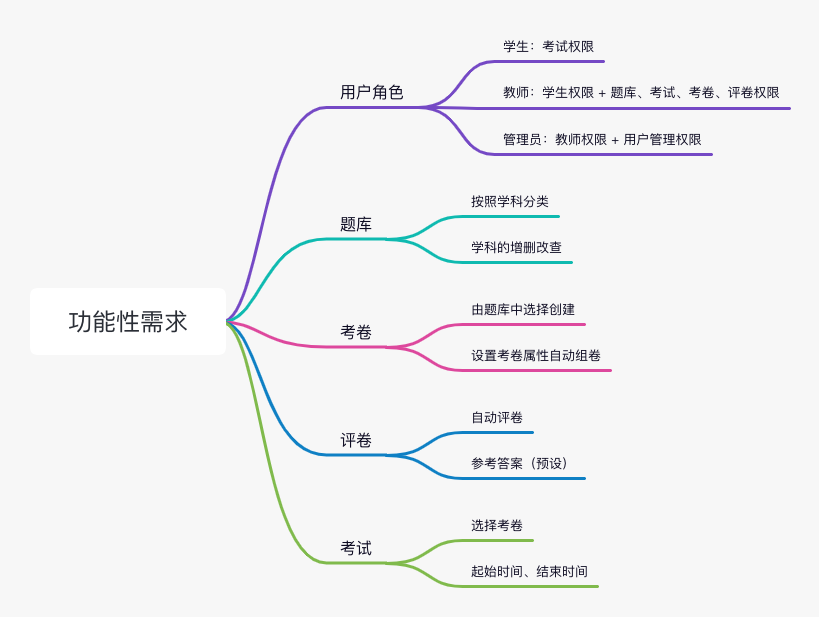
\includegraphics[width=0.8\linewidth]{_images/功能性需求.png}
    \caption{功能性需求}
    \label{功能性需求}
\end{figure}
\paragraph{用户角色分类} 系统的参与者主要分为三类:学生、教师、管理员,学生与教师对应实际业务场景中的角色,管理员是因系统的操作与非业务的操作而存在。\upcite{ref6}
\paragraph{题库功能} 题目作为考卷的基本单位,考卷就是多个题目的组成。项目需要题目的基本管理功能。题目按题型又将分为:单选题、多选题、判断题等。题目按照学科分类,因此又需要题库功能对不同的学科题目进行管理。
\paragraph{考卷功能} 考卷是考试进行的必要组成部分,考卷需要由教师手动从题库中选择,或是通过设定一定的规则从设定好的题库中抽取自动组卷。考卷也需要基本的增删改查功能。
\paragraph{考试功能} 考试通过选择已创建的考卷而开启,学生可以进入已创建的考试进行线上考试。考试也需要设置起始时间和结束时间属性。
\paragraph{评卷功能} 题目设置的时候提供对应的正确答案选项,使得在作答结束后能够通过正确答案与学生的作答情况自动评卷计分,并提供预先设置的参考题解给学生。
\paragraph{用户管理} 管理员才被允许对系统中的用户进行新增、删除、修改信息、查看。用户也可以对自己的基本信息做修改,例如修改密码、头像、昵称。
\paragraph{权限分类} 根据以上的用户角色分类和功能模块,需要将具体的功能模块访问限制与用户角色对应。学生只允许参与考试和查看自己考试的情况;老师具有学生的所有权限用于考卷的试测,此外需要考卷功能模块、题库功能模块、评卷功能模块的权限;管理员具有所有的功能模块权限,即老师的权限加上用户管理功能模块的权限。\upcite{ref3}

\subsection{非功能性需求}
\begin{itemize}
    \item 界面美观,布局简洁大方;
    \item 用户交互操作友好。用户意外的错误操作,或是发生运行时错误,应有合理的信息提示;
    \item 系统使用需要有清晰、完善的文档说明,项目代码注释完善、易读;
    \item 项目需要具有足够的测试性,以保证系统性能可用于实际环境;
    \item 项目结构设计良好、易于维护,并留存有一定后期功能拓展的空间;
    \item 用户操作具有完备的鉴权流程,防止非法操作;
    \item 前端布局弹性,根据不同的分辨率响应式渲染展示;
\end{itemize}

\subsection{章节小结}
本章从目标群体、用户目的、功能性和非功能性需求四个方面对项目的实际业务场景,以及用户的真实需求进行了全面分析和深入探究。

其中主要确定了本项目的核心用户为学校(或教育机构)、教师、学生。进而,围绕着这几个核心用户群体的用户表层需求,去进行深挖、探究其本质的用户需求。从而得出本章节中表述的「功能性需求」部分的总结归纳。除此以外,还基于用户的交互体验和友好性,结合时下主流系统的标准,归纳出项目的非功能性方面的需求。如上的分析都为了项目的前期进展做准备,进而更好的在之后的项目推进中进行系统的设计与开发。